\section{White Box Attacks} \label{s:whiteboxattacks}
	Currently, general-purpose white-box attacks on ensemble models do not exist; therefore, based on the work by \citeauthor{liu2016} \cite{liu2016} which found that white-box attacks created for a single model can be transferred to other models, attacks were constructed for specific CLAWs and their effectiveness was measured against other CLAWs and the entire FIST ensemble.

	These attacks were implemented using the Cleverhans library \cite{papernot2018cleverhans} using the \codeword{FastGradientMethod} (FGM) for non-targeted attacks and \codeword{SaliencyMapMethod} function for JSM (Jacobian-based Saliency Map) targeted attacks. The FGM attack is based on the work by \citeauthor{goodfellow2015} \cite{goodfellow2015}, and the JSM attack is based on the work by \citeauthor{papernot2018cleverhans} \cite{papernot2018cleverhans}.

	\subsection{FGM attacks} \label{s:whiteboxattacks:fgm}
		Based on our observations, FGM attacks conducted on a single CLAW are transferable to the FIST ensemble. Results for tests conducted with the MNIST Fashion database \cite{zalandoresearchFashionMNIST} can be observed in Figure \ref{f:whitebox:fgm:fashion} and tests conducted with the CIFAR-10 database \cite{krizhevsky2009} can be observed in Figure \ref{f:whitebox:fgm:cifar}. These figures demonstrate each base filter's accuracy, the classification accuracy against an FGM attack created for the filter, and the classification accuracy of the attack created for the filter when applied to the FIST ensemble. As evident from the results, attacks created for each filter are generally extremely transferable and often result in even higher classification accuracies when applied to the FIST model. Attacks created for the identity (unfiltered), Gaussian, edge detection, minimum, maximum, and median filters were all found to be even more effective when applied to the FIST ensemble. Understanding why this happens and improving DRAGONFIST's overall effectiveness against the FGM attack could be interesting topics for future research.
		\begin{figure}
			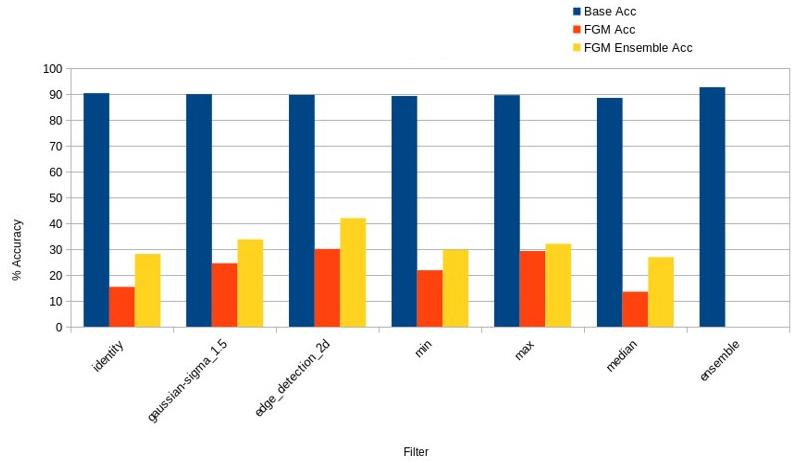
\includegraphics[width=\linewidth]{whitebox-fgm-fashion}
			\caption{White-box FGM attack on MNIST Fashion database.}
			\label{f:whitebox:fgm:fashion}
		\end{figure}
		\begin{figure}
			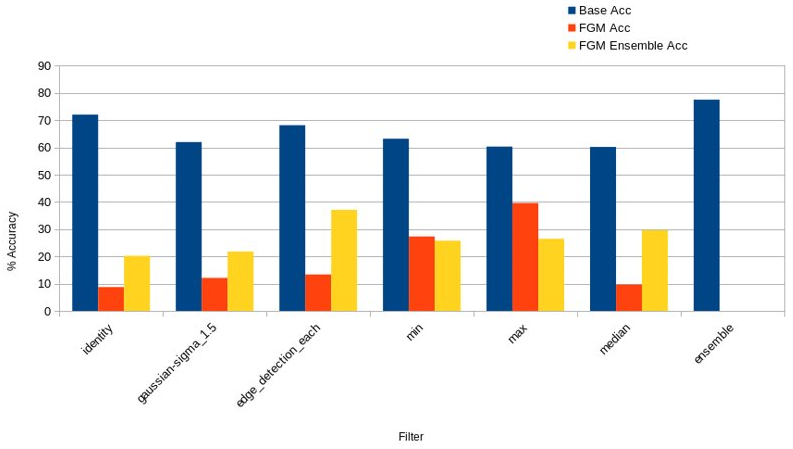
\includegraphics[width=\linewidth]{whitebox-fgm-cifar}
			\caption{White-box FGM attack on CIFAR database.}
			\label{f:whitebox:fgm:cifar}
		\end{figure}

	\subsection{JSM attacks} \label{s:whiteboxattacks:jsm}
		Based on our observations, contrary to what was observed in FGM attacks, JSM attacks conducted on a single CLAW are not nearly as transferable to the FIST ensemble. Results for the test conducted with the MNIST Fashion database \cite{zalandoresearchFashionMNIST} can be observed in Figure \ref{f:whitebox:jsm}. The figure demonstrates each filter's classification accuracy against a JSM attack and the classification accuracy of the attack created for the filter when applied to the FIST ensemble. As evident from the results, attacks created for each filter are not usually transferable to the FIST ensemble and the filters alone are often enough to stop the attack entirely. The edge detection, minimum, and median filters all observe \(0\%\) accuracy on adversarial images. This clearly highlights DRAGONFIST's effectiveness against the JSM attack.
		\begin{figure}
			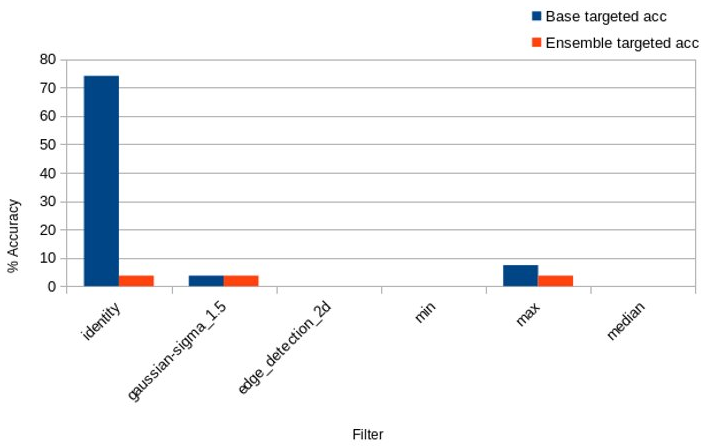
\includegraphics[width=\linewidth]{whitebox-jsm}
			\caption{White-box JSM attack on MNIST Fashion database.}
			\label{f:whitebox:jsm}
		\end{figure}
